\section*{Výsledky měření}
V SE modu jsme studovali lom slitiny Fe$_3$Al při dvou různých teplotách. Při pokojové teplotě (obrázek \ref{o:lom1}) nastal křehký intermetalický lom (podél hranic zrn). Při \SI{700}{\degreeCelsius} (obrázek \ref{o:lom2}) nastal vlivem vyšší difúze tvárný transkrystalický lom (skrz zrna).

V BSE modu jsme pomocí channelling kontrastu určili kruhovou metodou střední velikost zrna vzorku Ni (obrázek \ref{o:Ni}). "Dvojčata" jsme nepočítali jako jednotlivá zrna, stejně tak pokud byla krystalická plocha mírně deformovaná (to se na snímku projevilo intenzitním gradientem), tak jsme to ignorovali. Naměřená data jsou v tabulce \ref{t:kruhy}. Standardní odchylku každé kružnice odhadujeme na $\pm \SI{1}{zrno}$. Průměrná velikost zrna vychází ve všech snímcích přibližně stejná. Střední velikost zrna jsme spočítali ze všech kruhů. Předpokládáme, že rozdělení velikosti zrn je přibližně normální, standardní odchylku střední velikosti zrna jsme určili obvyklým způsobem
\begin{equation*}
\sigma_{\bar{d}}= \sqrt{\frac{1}{N(N-1)} \sum_{i=1}^{N}(d_i-\bar{d})^2  }=\SI{0.9}{\um} \,,
\end{equation*}
ke které jsme přes čtverec přičetli chybu jednoho měření.
Dostáváme střední velikost zrna
\begin{equation*}
\bar{d}=\SI{40.9(18)}{\um} \,.
\end{equation*}

V BSE modu jsme pozorovali pájku (slitina Pb a Sn), viz obrázek \ref{o:pajka}. Obrazovou analýzou snímku jsme určili poměr obou fází. V prvním snímku bylo \SI{29(1)}{\percent} Pb a \SI{69(2)}{\percent} Sn, ve druhém \SI{29(1)}{\percent} Pb a \SI{68(2)}{\percent} Sn (standardní odchylka je odhadnutá).
Pokud označíme tyto poměry $w_{\text{Pb}}$ respektive $w_{\text{Sn}}$, určíme frakční objem Pb následujícím způsobem (nejistota je určená metodou přenosu chyb)
\begin{equation*}
V_{Pb} \coloneqq \frac{w_{\text{Pb}}}{w_{\text{Pb}}+w_{\text{Sn}}}=\SI{29.7(10)}{\percent} \,.
\end{equation*}





\begin{tabulka}[htbp]
\centering
\begin{tabular}{c||ccc|c|c}
č. snímku & $D$ (\si{\um}) & č. kruhu & počet zrn & $d$ (\si{\um}) & $\bar{d}$ (\si{\um}) \\
\hline\hline
\multirow{5}{*}{1} & \multirow{5}{*}{219.1} & 1 & 27 & 38.2 & \multirow{5}{*}{38.1} \\ 
 &  & 2 & 27 & 38.4 &  \\ 
 &  & 3 & 29 & 35.9 &  \\ 
 &  & 4 & 27 & 38.8 &  \\ 
 &  & 5 & 27 & 38.9 &  \\ \hline
\multirow{5}{*}{2} & \multirow{5}{*}{238.7} & 1 & 25 & 45.0 & \multirow{5}{*}{43.9} \\ 
 &  & 2 & 23 & 49.1 &  \\ 
 &  & 3 & 30 & 37.8 &  \\ 
 &  & 4 & 26 & 43.8 &  \\ 
 &  & 5 & 26 & 44.0 &  \\ \hline
\multirow{5}{*}{3} & \multirow{5}{*}{227.4} & 1 & 32 & 33.5 & \multirow{5}{*}{38.8} \\ 
 &  & 2 & 29 & 37.1 &  \\ 
 &  & 3 & 30 & 36.0 &  \\ 
 &  & 4 & 24 & 45.2 &  \\ 
 &  & 5 & 26 & 41.9 &  \\ \hline
\multirow{5}{*}{4} & \multirow{5}{*}{229.6} & 1 & 23 & 47.0 & \multirow{5}{*}{43.3} \\ 
 &  & 2 & 23 & 47.2 &  \\ 
 &  & 3 & 26 & 42.0 &  \\ 
 &  & 4 & 29 & 37.8 &  \\ 
 &  & 5 & 26 & 42.3 &  \\ \hline
\multirow{5}{*}{5} & \multirow{5}{*}{244.6} & 1 & 27 & 42.7 & \multirow{5}{*}{40.5} \\ 
 &  & 2 & 29 & 39.9 &  \\ 
 &  & 3 & 35 & 33.2 &  \\ 
 &  & 4 & 26 & 44.9 &  \\ 
 &  & 5 & 28 & 41.8 &  \\ 


\end{tabular}
\caption{Kruhová metoda, pro každý kruh je spočtená velikost zrna $d$ podle \eqref{e:kruhy}, $\bar{d}$ je střední hodnota pro daný snímek.}
\label{t:kruhy}
\end{tabulka}

\begin{figure}[htbp]
\centering
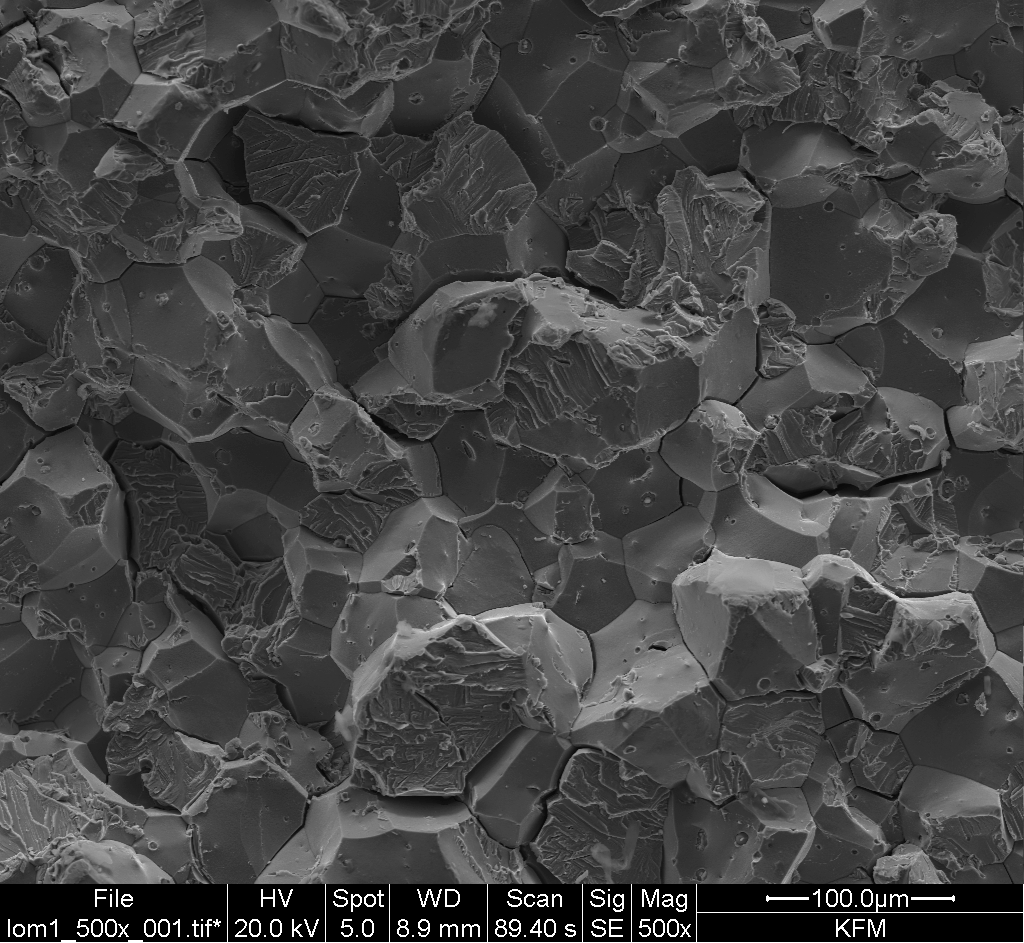
\includegraphics[width=\textwidth-6cm]{graficos/lom1.png}
\caption{Interkrystalický lom při pokojové teplotě}
\label{o:lom1}
\end{figure}

\begin{figure}[htbp]
\centering
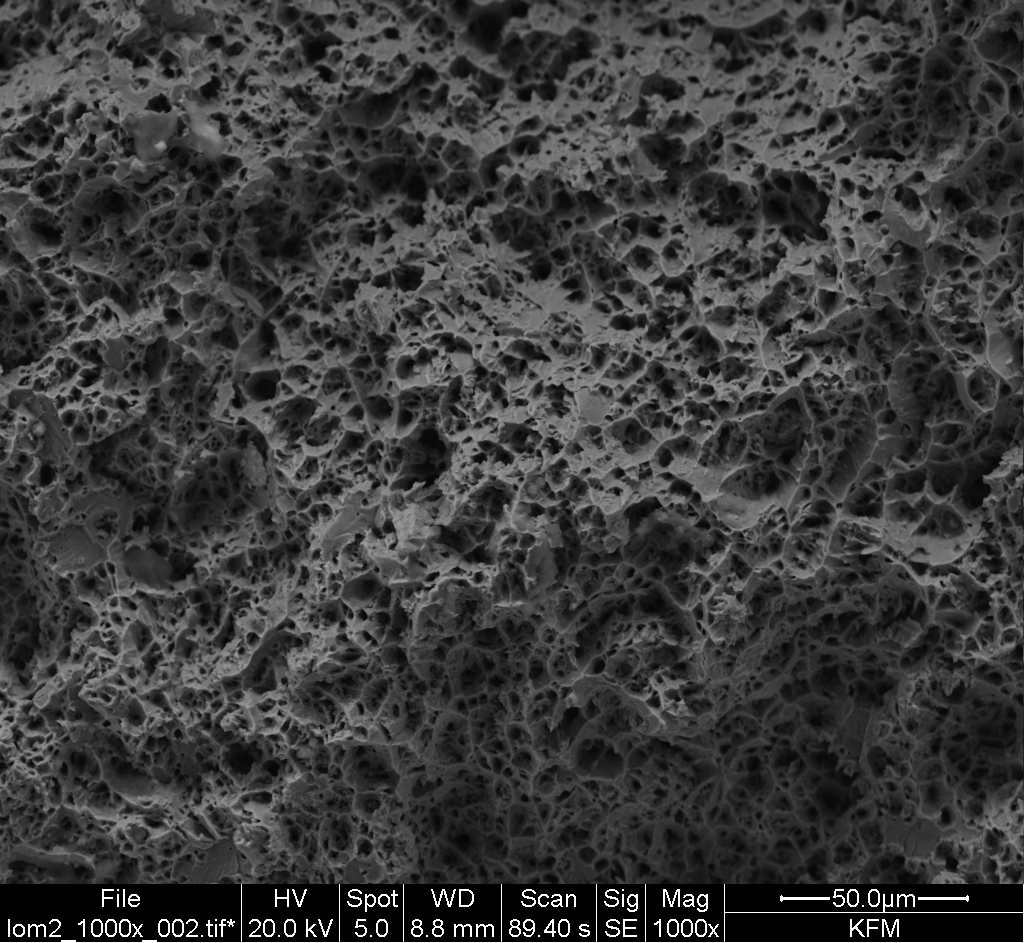
\includegraphics[width=\textwidth-6cm]{graficos/lom2.png}
\caption{Transkrystalický lom při \SI{700}{\degreeCelsius}}
\label{o:lom2}
\end{figure}

\begin{figure}[htbp]
\centering
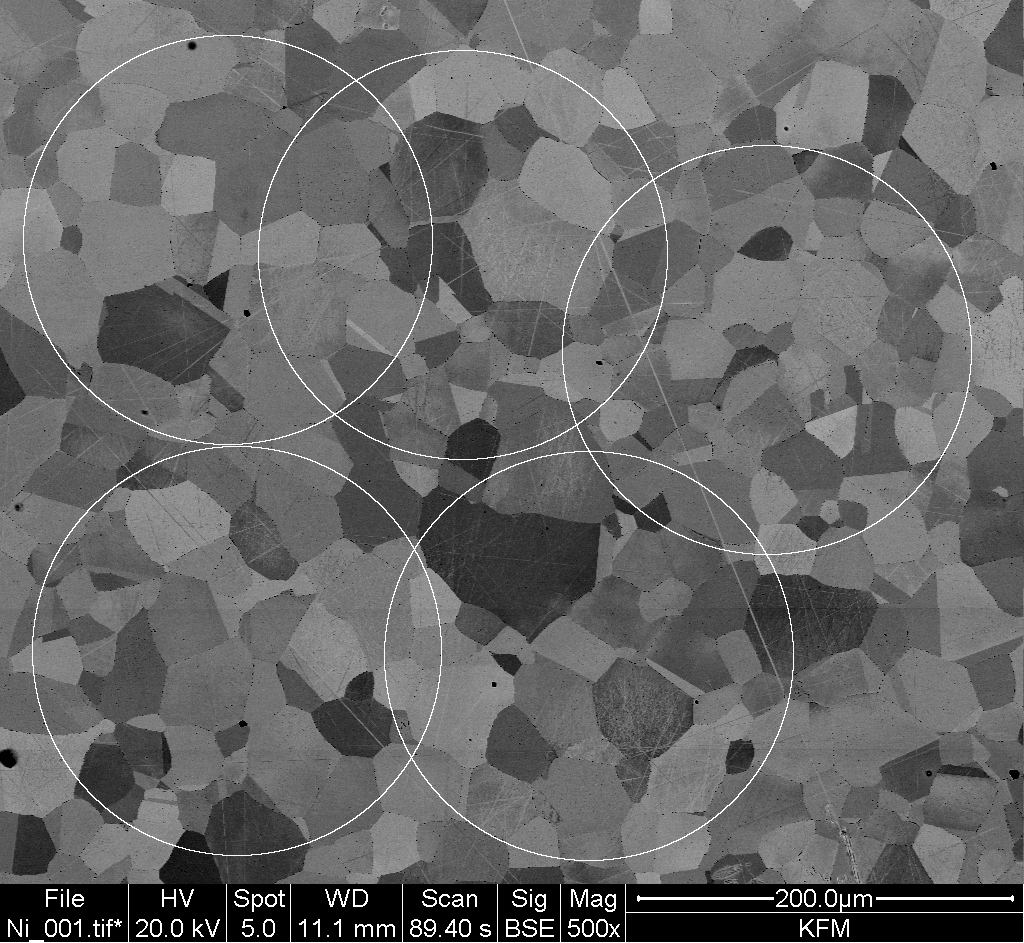
\includegraphics[width=\textwidth-6cm]{graficos/Ni_001.png}
\caption{Zrna niklu s různou orientací, znázorněná kruhová metoda (snímek č. 1, číslování kruhů začíná levým horním kruhem a pokračuje po směru hodinových ručiček).}
\label{o:Ni}
\end{figure}

\begin{figure}[t]
\centering
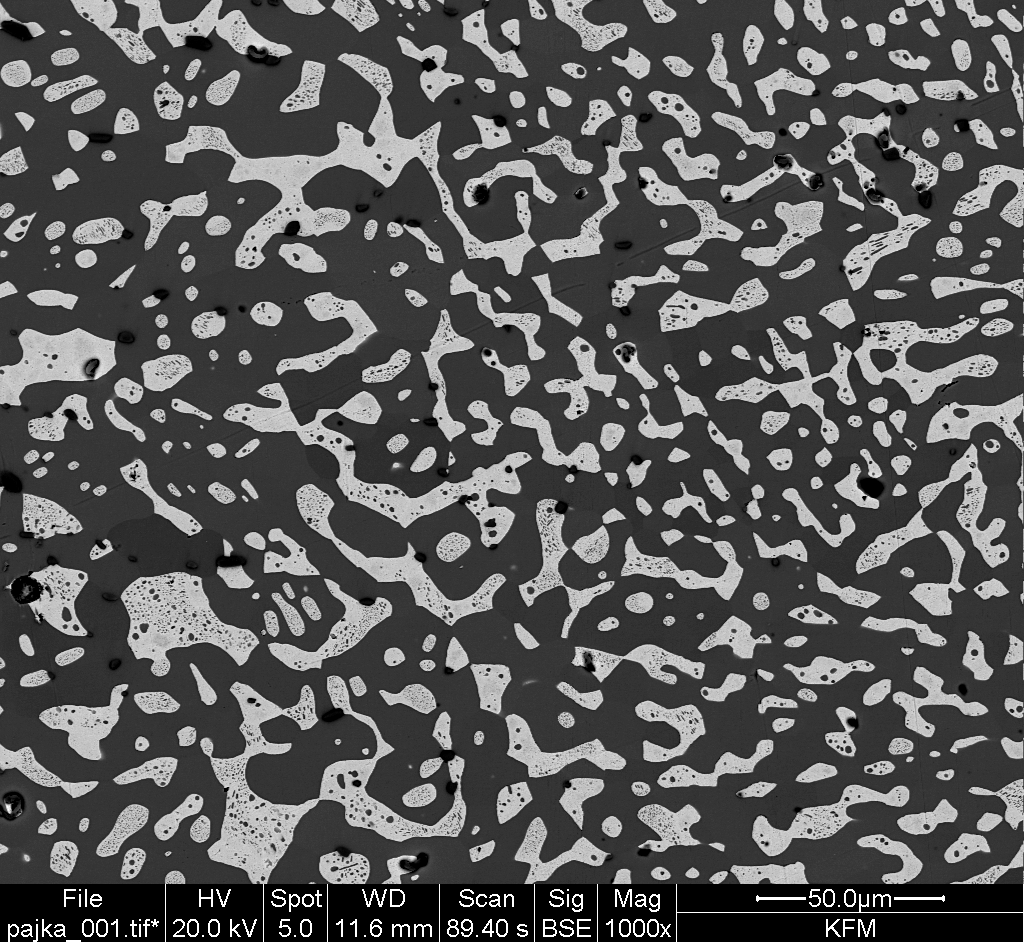
\includegraphics[width=\textwidth-6cm]{graficos/pajka1.png}
\caption{Pájka, slitina cínu (tmavě šedá) a olova (světle šedá).}
\label{o:pajka}
\end{figure}